\setlength{\emergencystretch}{2em}
% ReScience C replication of Lee & Zhang (ICLR 2025), arXiv:2504.12189v1.
% Every number labeled "replication" is computed from ../results/raw/*.csv (see ../results/*.md); every number labeled
% "original" is quoted from the original paper (Tables 2-4) or, where stated, from the authors' published result files.
\graphicspath{{../figures/}}
\newcommand{\LOO}{LOO-StabCP}
\newcommand{\RO}{RO-StabCP}
% expandable \input for generated table bodies (plain \input is not expandable inside tabular)
\makeatletter\newcommand{\inputtable}[1]{\@@input #1 }\makeatother

\section{Introduction}

Conformal prediction (CP) turns any point predictor into a set-valued predictor whose coverage holds in finite
samples and without distributional assumptions, provided the data are exchangeable\supercite{vovk2005algorithmic}.
The price of this guarantee is computation. For each test input and each candidate outcome, \emph{full} conformal prediction augments all labeled training examples with that single input--outcome pair and refits the model. It does not fit all test points together. \emph{Split} conformal prediction\supercite{papadopoulos2002inductive,lei2018distribution} instead fits the model once on a training portion of the labeled sample and reserves the remaining labeled examples solely to calibrate the score quantile. Those calibration examples are not discarded, but they are not used to fit the model. This reduces computation at the cost of fitting on fewer examples, and the resulting intervals can vary from one random split to the next.

Stability-based conformal prediction offers a middle way. Ndiaye\supercite{ndiaye2022stable} observed that if the
fitted model changes little when one observation is \emph{replaced}, then the nonconformity scores of every
candidate label can be bounded using a single fit, inflated by an algorithmic-stability bound. The resulting
replace-one method (\RO) still needs one fit per test point. Lee and Zhang\supercite{lee2025loo} propose
\emph{leave-one-out} stable conformal prediction (\LOO). It uses a stability bound for \emph{adding or removing} one
observation, so a single model fitted on the training data serves all $m$ test points. The paper proves finite-sample
validity, derives explicit bounds for regularized M-estimation (RLM) and stochastic gradient descent (SGD), proposes
heuristic bounds for neural networks, and applies the method to conformal screening with false discovery rate (FDR)
control. The central empirical question is whether this reduction in fitting cost preserves coverage while producing intervals of competitive length.

This study examines the reproducibility of these empirical claims through an independent Python implementation and a comparison of three sources: the arXiv v1 paper, the authors' public repository, and the ICLR 2025 supplementary material. The distinction matters because these sources specify different experimental settings. The initial implementation and primary experiments were based on the paper; the repository and supplement were subsequently used to diagnose discrepancies. The kernel implementation was added after consulting the supplement and is not independent of that source.

The contributions are threefold. First, the study evaluates eight claims across the synthetic, real-data, neural-network, kernel, derandomization and screening experiments. Second, it separates results obtained from the interpretation of the paper adopted here from results obtained using settings recovered from the authors' code. Third, it examines the consequences of feature scaling, the kernel representation and a discrepancy in the screening stability bound through controlled variants.

The outcome is a \emph{partial replication}. The coverage and computational comparisons for the linear models support the original claims, but shorter intervals than split CP are not obtained uniformly. Neural-network and kernel results depend on settings recovered from the supplementary code. The derandomization comparison changes under the text-based settings, and the screening power advantage over cfBH does not persist when the stability bound is computed as stated in the paper. These conclusions concern the experiments and implementations studied here, not a refutation of the underlying conformal-validity theorem. Table~\ref{tab:verdicts} summarizes the claim-level evidence.

\section{Scope of reproducibility}
\label{sec:scope}

The study tests eight claims. The wording in quotation marks is taken from the original paper; the claim numbering is specific to this replication.

\begin{description}
\item[C1 Validity.] \LOO\ attains marginal coverage of at least $1-\alpha=0.9$ (Theorem~1; Tables~2 and~3 of the
  original). Empirical coverage is assessed relative to 0.9, with sampling uncertainty reported; finite experiments cannot establish the theorem for other data distributions.
\item[C2 Accuracy.] \LOO\ is ``competitive'', with lengths ``comparable to OracleCP, FullCP, RO-StabCP'', and
  ``SplitCP continues to produce more variable and lengthier prediction intervals compared to most other methods''
  (§4--§5). \emph{Supported if} mean length is close to FullCP and \RO, and both the mean and the standard
  deviation of the length are smaller than SplitCP's.
\item[C3 Speed.] \LOO\ is ``on par with SplitCP'' in runtime and much faster than \RO\ and FullCP, and the gap
  to \RO\ grows with the number of test points $m$ (§4--§5). \emph{Supported if} this ordering holds in the replication
  timings.
\item[C4 SGD.] For SGD the leave-one-out bound is half the replace-one bound, so \LOO\ intervals are shorter than
  \RO\ intervals; for RLM the two are nearly equal (Theorem~3; Table~2 of the original).
\item[C5 Neural networks.] With the heuristic bound of Eq.~(8), \LOO\ remains valid for neural networks and gives
  intervals comparable to the baselines at a fraction of \RO's cost (Fig.~3 of the original; App.~A.2).
\item[C6 Kernels.] Kernel RLM and SGD keep coverage and give shorter intervals in the nonlinear setting (App.~A.1).
\item[C7 Derandomization.] \LOO\ is less conservative and faster than derandomized split CP
  (MM-SplitCP\supercite{solari2022multi} and EM-SplitCP\supercite{gasparin2024merging}; App.~B).
\item[C8 Screening.] LOO-cfBH controls the FDR, ``is more powerful'' than cfBH\supercite{jin2023selection}
  and is ``less conservative and more powerful compared to RO-cfBH'', while being much faster than RO-cfBH (§6;
  Table~4 of the original).
\end{description}

All eight claims were evaluated within the experimental configurations specified below; the theoretical guarantees were not independently re-proved. C6 was not attempted until the authors' supplementary material became available: the paper
does not define the feature map used for the kernels inside the stability bounds, and the public repository contains
no kernel experiment. The supplement's \texttt{kernel.py} supplies the missing choices (Section~\ref{sec:kernel}).
Beyond the qualitative claims, the study also examines whether the \emph{numbers} in the original tables can be
reproduced.

Verdicts describe the tested settings rather than universal guarantees. Four categories are used. \emph{Reproduced}: the empirical evidence supports the claim within this scope. \emph{Reproduced with qualification}:
the claim holds, but only under choices not stated in the paper, or with an explicitly stated caveat. \emph{Partially
reproduced}: some parts of a compound claim hold and others do not. \emph{Not reproduced}: the claim does not hold in
replication runs.

\section{Background}
\label{sec:background}

Let $D=\{(X_i,Y_i)\}_{i=1}^n$ be training data and $X_{n+1},\dots,X_{n+m}$ test inputs, all exchangeable with the
unseen responses. A prediction set $C(X_{n+j})$ is \emph{valid} if
\begin{equation}
  \Pr\big(Y_{n+j}\in C(X_{n+j})\big)\ \ge\ 1-\alpha .
  \label{eq:validity}
\end{equation}
All methods use the absolute-residual score $S(y,\hat y)=|y-\hat y|$. For a finite multiset $A$,
$Q_{1-\alpha}(A)$ denotes its $\lceil(1-\alpha)|A|\rceil$-th smallest element.

\paragraph{Full and split CP.} Let $\hat f^{y}$ be the model fitted on $D\cup\{(X_{n+j},y)\}$ and
$S_i^y=S(Y_i,\hat f^y(X_i))$, with $S^y_{n+1}$ the score of the candidate itself. Full CP returns
\begin{equation}
  C^{\mathrm{full}}(X_{n+j})=\Big\{y:\ S^y_{n+1}\le Q_{1-\alpha}\big(\{S_i^y\}_{i=1}^n\cup\{\infty\}\big)\Big\},
  \label{eq:fullcp}
\end{equation}
which requires one fit per candidate $y$ for each test input, in practice per point of a grid. Split CP partitions $D$ into disjoint training and calibration subsets, fits only on the training subset, and uses the held-out calibration scores to determine the quantile. OracleCP is the infeasible full CP that
uses the true $Y_{n+j}$; it serves as a lower reference for length.

\paragraph{Replace-one stability (\RO).} Fit once per test point on $D\cup\{(X_{n+j},\tilde y_j)\}$ with an
arbitrary guess $\tilde y_j$, giving $\hat f_j^{\tilde y}$ and scores $S_{i,j}^{\tilde y}$. If replacing the guessed
label by any other label changes each score by at most $\tau^{\mathrm{RO}}_{i,j}$, then
\begin{equation}
  C^{\mathrm{RO}}(X_{n+j})=\Big\{y:\ |y-\hat f_j^{\tilde y}(X_{n+j})|-\tau^{\mathrm{RO}}_{n+j,j}\le
  Q_{1-\alpha}\big(\{S^{\tilde y}_{i,j}+\tau^{\mathrm{RO}}_{i,j}\}_{i=1}^n\cup\{\infty\}\big)\Big\}
  \label{eq:ro}
\end{equation}
contains the full-CP set and is therefore valid\supercite{ndiaye2022stable}.

\paragraph{Leave-one-out stability (\LOO).} Let $\hat f$ be fitted on $D$ only and $S_i=S(Y_i,\hat f(X_i))$. An
algorithm is leave-one-out stable with bounds $\tau^{\mathrm{LOO}}_{i,j}$ if
\begin{equation}
  \sup_{y,z}\ \big|S\big(z,\hat f_j^{y}(X_i)\big)-S\big(z,\hat f(X_i)\big)\big|\ \le\ \tau^{\mathrm{LOO}}_{i,j},
  \qquad i\in\{1,\dots,n\}\cup\{n+j\}.
\end{equation}
Algorithm~1 of the original then returns the interval
\begin{equation}
  C^{\mathrm{LOO}}(X_{n+j})=\hat f(X_{n+j})\ \pm\ \Big\{Q_{1-\alpha}\big(\{S_i+\tau^{\mathrm{LOO}}_{i,j}\}_{i=1}^n
  \cup\{\infty\}\big)+\tau^{\mathrm{LOO}}_{n+j,j}\Big\},
  \label{eq:loo}
\end{equation}
which again contains the full-CP set (Theorem~1 of the original). Only $\hat f$ is fitted; the $m$ test points differ
only through the bounds.

\paragraph{Stability bounds.} The original gives explicit bounds for a linear model $f_\theta(x)=x^\top\theta$
trained with a $\gamma$-Lipschitz loss; the experiments use the Huber loss with $\epsilon=1$, so $\gamma=\epsilon=1$.
Write $\nu_i=\|X_i\|$ and $\rho_{n+j}=\|X_{n+j}\|$, and let $\bar\rho$ be the mean of $\nu_1,\dots,\nu_n$. For RLM,
$\hat\theta=\arg\min_\theta \tfrac{1}{N}\sum_i \ell(Y_i,X_i^\top\theta)+\Omega(\theta)$, where $\Omega$ is
$\lambda$-strongly convex, the bounds used in the experiments (App.~G.1 of the original) are
\begin{equation}
  \tau^{\mathrm{LOO}}_{i,j}=\frac{2\gamma\,\nu_i\,(\rho_{n+j}+\bar\rho)}{\lambda(n+1)},\qquad
  \tau^{\mathrm{RO}}_{i,j}=\frac{4\gamma\,\nu_i\,\rho_{n+j}}{\lambda(n+1)} .
  \label{eq:rlmbound}
\end{equation}
For SGD with random reshuffling, $R$ epochs and step size $\eta$ (Algorithm~9 of the original), the bounds are
\begin{equation}
  \tau^{\mathrm{LOO}}_{i,j}=R\,\eta\,\gamma\,\nu_i\,\rho_{n+j},\qquad
  \tau^{\mathrm{RO}}_{i,j}=2R\,\eta\,\gamma\,\nu_i\,\rho_{n+j},
  \label{eq:sgdbound}
\end{equation}
so the leave-one-out bound is exactly half the replace-one bound, which is the basis of claim C4. The original
derives these bounds with the expansiveness property of gradient updates from the stability analysis of SGD by Hardt
et al.\supercite{hardt2016train} (their Lemma~3.6). For neural networks the original proposes the
heuristic $\tau\approx R\eta\gamma\|X_i\|\|X_{n+j}\|$ (Eq.~(8)), with the replace-one version again twice as large.

\paragraph{Conformal screening.} Given test points with thresholds $c_j$, cfBH\supercite{jin2023selection} tests
$H_{0j}: Y_{n+j}\le c_j$ with the monotone score $S(y,\hat y)=100y-\hat y$ and split-conformal p-values
\begin{equation}
  p^{\mathrm{split}}_j=\frac{\sum_{i\in I_{\mathrm{calib}}}\mathbb 1\{S_i<S^{c_j}_{n+j}\}+1}{|I_{\mathrm{calib}}|+1}.
\end{equation}
LOO-cfBH replaces them by full-data p-values whose scores are widened by the leave-one-out bounds (Eq.~(7) of the
original):
\begin{equation}
  p^{\mathrm{LOO}}_j=\frac{\sum_{i=1}^n\mathbb 1\{S_i-\tau_{i,j}<S^{c_j}_{n+j}+\tau_{n+j,j}\}+1}{n+1}.
  \label{eq:loop}
\end{equation}
Both are passed to the Benjamini--Hochberg procedure\supercite{benjamini1995controlling}: with
$k^*=\max\{k:\sum_j\mathbb 1\{p_j\le qk/m\}\ge k\}$, the hypotheses with the $k^*$ smallest p-values are rejected.
RO-cfBH uses replace-one bounds and one fit per test point.

\section{Methodology}
\label{sec:methods}

\subsection{Implementation}

The methods were implemented in Python with numpy, numba and scikit-learn, without cvxpy or a deep-learning framework. The initial implementation was based on the arXiv v1 text (PDF and \LaTeX{} source). Functions carry comments naming the algorithms, equations or sections implemented, and choices left open by the paper are marked as assumptions with their rationale; these choices are listed in Appendix~\ref{app:assumptions}. The author states that the primary experiments were run and committed in a private archive before the authors' repository\supercite{authorscode} was consulted for diagnosis (commit \texttt{3b37682}, 14~February~2025 UTC). This public repository is a sanitized snapshot with new git history. Those private pre-diagnosis commits and tags are not in this repository, and tags on GitHub do not substantiate that chronology. Relevant behaviors were subsequently implemented as separately named diagnostic options. The use of an AI tool in preparing the replication is disclosed in the Discussion.

The ICLR 2025 supplementary material\supercite{leezhang2025supp} was obtained later. This 1.1~MB archive (SHA-256 \texttt{7f39cd75\allowbreak fda4e126\allowbreak ebdf5f54\allowbreak 5b34c3db\allowbreak e2208f62\allowbreak 16086e41\allowbreak 37f23ef8\allowbreak 2a765e53}) holds an earlier, fuller version of the code than the repository: scripts for every experiment of the paper, including the neural networks (\texttt{real\_NN.py}), kernels (\texttt{kernel.py}) and derandomized baselines (\texttt{synthetic\_derandom.py}, \texttt{real\_derandom.py}), together with their raw result files (seven CSV files) and figures. Like the repository, the supplement was used to explain differences, with source-derived choices tagged in the replication code. The kernel code (Section~\ref{sec:kernel}) was written after the supplement was consulted and is therefore not a clean-room implementation. In this article, ``the authors' code'' means the repository and the supplement together; differences between the two are identified explicitly.

\paragraph{Models.} The linear regression experiments use $f_\theta(x)=x^\top\theta$ without intercept and the Huber loss
with $\epsilon=1$. RLM uses $\Omega(\theta)=\|\theta\|^2$ and is solved to numerical optimality
($\|\nabla\|<10^{-10}$) by a damped Newton method; the authors' code solves it with cvxpy\supercite{diamond2016cvxpy}.
The paper never states the numerical value of $\lambda$ in Eq.~(\ref{eq:rlmbound}). The replication uses $\lambda=2$, the
strong-convexity constant of $\|\theta\|^2$; the authors' code also uses \texttt{lamb=2}. (The definition of
strong convexity in §3.2.1 of the original appears to omit the usual $t(1-t)$ factor, interpreted here as a typographical error.) As a
sensitivity check the RLM bounds were also computed with $\lambda=1$, which doubles them. SGD uses
$\theta_0=0$, $R=15$ epochs (5 for FullCP, as stated in the paper) and $\eta=0.001$. The neural networks have one
hidden layer of 20 sigmoid units (Fig.~3 of the original) or two hidden layers of 10 and 5 units (App.~A.2), a linear
output, Huber loss, Glorot-uniform initialization, per-sample SGD, $R=30$ and $\eta=0.001$. The authors' setup
replaces this network by the one the supplement trains (D17--D19 in Table~\ref{tab:diffs}). For the kernel study
(App.~A.1 of the original) each point $x$ is represented by its kernel row $(k(x,X_1),\dots,k(x,X_n))$ with the $n$
training points as centers, and the linear model is fitted to these features, by SGD and, in the text setup only, by
RLM with penalty $\theta^\top K\theta$.

\paragraph{Conformal details.} FullCP evaluates 100 equally spaced candidates on $[\min y-r/4,\ \max y+r/4]$, where
$r$ is the range of the training responses; the interval length is the number of accepted candidates times the grid
step. SplitCP uses a 70/30 split. \RO\ uses $\tilde y_j=$ mean of the training responses. MM-SplitCP and EM-SplitCP
combine $K=30$ split-conformal intervals at level $1-\alpha/2$ by a majority vote and by the running exchangeable
majority vote of Gasparin and Ramdas\supercite{gasparin2024merging}, respectively. The authors' setup uses $K=50$
on real data, as the supplement does (D10).

\subsection{Data and experiments}

\begin{description}
\item[Synthetic data (§4).] $n=m=100$, $d=100$. The paper specifies $X\sim N(0,\Sigma/d)$ with
  $\Sigma_{kl}=0.5^{|k-l|}$, $\beta_k\propto(1-k/d)^5$ scaled to $\|\beta\|^2=d$, and $Y=\mu(X)+N(0,1)$ with
  $\mu(x)=x^\top\beta$ (linear) or $\mu(x)=\sum_k\beta_k\exp(x_k/10)$ (nonlinear). 100 repetitions.
\item[Real data (§5).] Boston Housing\supercite{harrison1978hedonic} ($506\times13$) and
  Diabetes\supercite{efron2004least} ($442\times10$). The paper states that ``all continuous variables have been
  normalized''; every column, including the response, is z-scored in the replication. $m\in\{1,100\}$ points are held out at random and
  the rest are used for training; 100 repetitions. Boston Housing was removed from scikit-learn, so the replication uses a widely
  mirrored copy of the original table, fixed by checksum.
\item[Neural networks (§5, App.~A.2).] The same real-data sets, $m=100$ (the paper does not state $m$; the
  granularity of the coverage boxes in Fig.~3 of the original implies $m=100$), 100 repetitions, comparing SplitCP,
  \RO\ and \LOO.
\item[Kernels (App.~A.1).] The two synthetic settings of §4, each without a kernel, with the RBF kernel
  $\exp(-\|x-x'\|^2/(2\sigma^2))$, $\sigma=0.1$, and with the polynomial kernel $(x^\top x'+1)^2$; SplitCP, \RO\
  and \LOO; 100 repetitions.
\item[Derandomized baselines (App.~B).] MM-SplitCP and EM-SplitCP added to the synthetic and real-data runs
  ($m=100$).
\item[Screening (§6).] The Campus Recruitment data\supercite{roshan2020placement} (215 candidates). The response is
  placement (0/1); \texttt{salary} is dropped because it exists only for placed candidates, and the seven categorical
  features are dummy-coded (14 features in total). The setup holds out 20\% (43 candidates) as test points, sets $c_j=0$, fits
  the linear Huber model by SGD ($R=15$, $\eta=0.001$) and uses $q\in\{0.1,0.2,0.3\}$; 1000 repetitions. The paper
  states that the regression set-up of §5 is ``imported''.
\end{description}

Each repetition draws its data, splits and SGD shuffles from a generator seeded by a fixed master seed. Coverage is
the fraction of the $m$ test points covered in a repetition; length is the mean interval length over the $m$ points;
time is the wall-clock time of one method on one repetition (all fits, bounds and intervals). FDP is the number of false rejections divided by the total number of rejections, or zero if there are none. Power is the fraction of true alternatives rejected, set to zero if no alternatives are present. FDR is the expectation of FDP; it is estimated by the mean FDP over repetitions. Lower length is preferable only in conjunction with adequate coverage; higher power is preferable only in conjunction with FDR control. Tables report means unless stated otherwise. Standard deviations (SDs) describe variation between repetitions, not uncertainty in a mean.

\paragraph{Uncertainty and comparisons.} For independent repetitions the standard error (SE) of a mean is its sample SD divided by the square root of the number of repetitions. When comparing methods on the same repetition, the SE is instead computed from the paired differences (Table~\ref{tab:c2}). Screening runs following the authors' split schedule are clustered by train/test split, so uncertainty is based on the ten split-level means rather than treating 1000 repetitions as independent. Comparisons with the authors' files use different random realizations and are reported as absolute or relative numerical differences, not as assertions of statistical equivalence. No equivalence margin or multiple-comparison testing procedure was specified; small differences should therefore not be interpreted as proof of equality.

\subsection{Two named setups}
\label{sec:setups}

The initial runs followed the documented interpretation of the text and did not reproduce the published numbers. Reading the authors' code
and supplementary material showed several choices that the paper does not report. Every regression and screening experiment is therefore reported
under two setups, used throughout:

\begin{description}
\item[Text setup.] The interpretation of the paper adopted here, with the choices of Appendix~\ref{app:assumptions} wherever the text is silent. This is one defensible implementation, not the only possible reading. For kernels, even this setup uses the feature map recovered from the supplement.
\item[Authors' setup.] The text setup plus every unreported choice from the authors' code that affects the
  experiment (Table~\ref{tab:diffs}). This is the diagnostic reconstruction of what produced the original tables.
\end{description}

Table~\ref{tab:diffs} lists the identified differences between the paper text and the authors' code. Each row gives
what the paper says (or the interpretation adopted here where it is silent), what the code does, and the measured effect of an isolated or explicitly grouped switch where available. Some entries are descriptive rather than separately isolated ablations. Two rows dominate: the synthetic data-generating process
(D1) and the scaling of real-data features (D2). The analogous feature scaling in screening (D13) and a missing
factor in one screening bound (D14) are the two rows that matter for C8.

\begin{table}[htbp]
\centering\scriptsize
\caption{Differences between the paper text and the authors' code: the repository at commit \texttt{3b37682} and,
for rows marked S, the ICLR supplementary material. ``Effect'' is the change in replication results when only that item (or the
items named) is switched from the text to the code version. Coverage and length are means over 100 repetitions;
power is the mean over 1000 repetitions. The authors' setup includes every row except D8, D9, D11 and D20, which are not
data or method choices.}
\label{tab:diffs}
\begin{tabular}{@{}l >{\raggedright\arraybackslash}p{2.9cm} >{\raggedright\arraybackslash}p{3.6cm} >{\raggedright\arraybackslash}p{5.3cm}@{}}
\toprule
ID & Paper text (or the interpretation adopted here) & Authors' code & Effect of switching to the code version \\
\midrule
D1 & Synthetic $\|\beta\|^2=d$ & S: $\|\beta\|^2=1/d$, so the signal variance is about $10^{-4}$; same AR(1)
  design as the text (the later repository version also drops AR(1)) & Explains all synthetic lengths: linear RLM
  \LOO\ length 6.515 $\to$ 3.371 (original 3.442); the supplement's result file equals Table~2 \\
D2 & Real features z-scored, $\|X_i\|\approx\sqrt d$ & z-scored, then divided by $\sqrt d$, so $\|X_i\|\approx1$ &
  Explains the real-data and neural-network lengths: Boston SGD \LOO\ length 2.284 $\to$ 1.841, coverage 0.961 $\to$
  0.898 \\
D3 & SGD fits draw independent shuffles & One set of $R$ shuffles per repetition, shared by all fits & None
  (third decimal) \\
D4 & \RO\ guess $\tilde y=$ mean of $y$ & $\tilde y=0$ & Small (with D5: Boston RLM \RO\ length 2.195 $\to$ 2.174) \\
D5 & $Q_{1-\alpha}$ of $n$ scores plus $\infty$ & ``higher'' empirical quantile, no $\infty$ & One rank lower when
  $n\ne100$; slightly shorter intervals \\
D6 & FullCP grid unspecified (replication: 100 points, $\pm r/4$) & 100 points on $[\min y-\mathrm{sd},\max y+\mathrm{sd}]$;
  interval from first to last accepted point & FullCP under-covers slightly (Boston RLM coverage 0.898 $\to$ 0.890),
  as in the original \\
D7 & Split size $0.7n$, rounded & $\lfloor0.7n\rfloor$ & Small (with D5: Boston RLM SplitCP length 2.017 $\to$
  1.916) \\
D8 & RLM ``solved using gradient descent'' & cvxpy & Absolute run times only \\
D9 & $\lambda$ not stated & $\lambda=2$ & None (same as replication) \\
D10 & Derandomized baselines: $K=30$ & S: D5 at level $1-\alpha/2$; $K=50$ on real data & D5: linear RLM MM-SplitCP
  length 4.579 $\to$ 3.851; $K$: at most 0.085 \\
D11 & Neural networks & S only: \texttt{real\_NN.py}, \texttt{results\_nn.csv} & See D2, D17--D20 \\
D12 & Screening: 20\% test, new split per repetition & 30\% test; split redrawn only every 100th repetition, so 10
  distinct splits in 1000 & Means move by up to 0.05; ignoring split clustering understates the reported power SEs by about tenfold \\
D13 & Screening: continuous features z-scored, no intercept & All columns z-scored, divided by $\sqrt{p+1}$,
  constant column added & Main cause of the power gap: LOO-cfBH power at $q=0.1$ 0.185 $\to$ 0.602 \\
D14 & LOO-cfBH training bound $R\eta\gamma\nu_i\rho_{n+j}$ (App.~G.1) & Factor $R=15$ missing
  (\texttt{funcs/CP\_screening.py}, line 122) & Inflates LOO-cfBH power; correcting it lowers power at $q=0.1$ from
  0.608 to 0.483 \\
D15 & cfBH: 70/30 split & 50/50 split & Small (cfBH power at $q=0.1$: 0.660 $\to$ 0.679) \\
D16 & BH rejects $p_j<qk^*/m$; RO-cfBH $\tilde y=$ mean; p-values once per repetition & ``$\le$''; $\tilde y=0$;
  shared shuffles; each method re-run per $q$ & Not isolated; included in the authors' setup \\
D17 & NN: sigmoid units & S: ReLU (the \texttt{'logistic'} key is never read) & Not isolated from D18 \\
D18 & NN: SGD as in §3.3, Huber loss & S: scikit-learn \texttt{MLPRegressor}: squared loss, mini-batches of 200,
  momentum 0.9, L2 $10^{-4}$, early stop, the same seed (42) for every fit & With D17: Diabetes (10,5) \LOO\ length
  3.254 $\to$ 3.050 \\
D19 & NN bound Eq.~(8), $R\eta\|X_i\|\|X_{n+j}\|$ & S: constant $R\eta$ (\LOO), $2R\eta$ (\RO) & At most 0.034 in
  length (given D2) \\
D20 & NN figures: one and two hidden layers & S: one result file, the (10,5) run; script set to (20) & What can be
  compared (Section~\ref{sec:nn}) \\
D21 & Kernel: RBF $\sigma=0.1$ ($\gamma=50$) & S: $\gamma=0.1$ ($\sigma\approx2.24$) & With D22: see below \\
D22 & Kernel: $\eta$ not stated (replication 0.001); RLM and SGD & S: $\eta=10^{-5}$; SGD only & With D21: linear poly
  \LOO\ coverage 1.000 $\to$ 0.900, length 11.575 $\to$ 6.541 \\
\bottomrule
\end{tabular}
\end{table}

The repository contains no code for the neural networks, kernels or derandomized baselines; the supplement does,
and the authors' setup for those experiments follows it (D10, D17--D22). In particular, MM- and EM-SplitCP in the
authors' setup apply the code's quantile rule (D5) to each split-conformal interval at level $1-\alpha/2$, as the
supplement's \texttt{MultiSplitCP} does.

\subsection{Reference values}

The original reports coverage, length and time for the synthetic study (Table~2), coverage only for the real data
(Table~3), FDR, power and time for screening (Table~4), and box plots only for the neural networks, kernels and
derandomized baselines. For the box plots, reference values come from the authors' raw result files in the
supplement\supercite{leezhang2025supp}: \texttt{results\_\allowbreak nn.csv} (two-layer networks, Fig.~6),
\texttt{results\_\allowbreak kernel.csv} (Fig.~5) and \texttt{results\_\allowbreak synthetic\_derandom.csv} and
\texttt{results\_\allowbreak real\_derandom.csv} (Figs.~7--8). As a check, the supplement's
\texttt{results\_\allowbreak synthetic\_ar1\_05.csv} equals every cell of Table~2 after rounding. Real-data reference lengths come from the repository's
\texttt{result/\allowbreak results\_\allowbreak real.csv}\supercite{authorscode}, which reproduces Table~3's
coverage. No raw result file was found for the one-layer networks of Fig.~3 in these materials (D20); their reference medians were digitized
from the figure in the arXiv source, with an accuracy of about 0.015 length units (Appendix~\ref{app:digitise}).

\subsection{Computational requirements}

All experiments ran on a shared Intel Xeon machine with 8 virtual CPUs, using 4 worker processes and a single BLAS
thread per process; no GPU was used. The software was Python~3.13.5, numpy~2.5.4, numba~0.68.0,
scikit-learn~1.9.1, scipy~1.18.1, pandas~3.1.0 and matplotlib~3.11.2. The full pipeline, including every variant
reported here, takes about 36 minutes (2169~s of logged experiment time, of which the neural networks take 1324~s
and the kernels 13~s; each screening variant takes a few seconds). Per-experiment times are listed in Appendix~\ref{app:compute}.

\section{Results}
\label{sec:results}

Results are reported claim by claim. Each subsection presents the evidence and ends with a verdict.

\subsection{Coverage and length on synthetic data (C1, C4)}

Table~\ref{tab:sim} compares the replicated synthetic results with Table~2 of the original. For each method it gives the mean
coverage and mean length over 100 repetitions under the text setup, under the authors' setup and in the original.
Under the text setup the mean coverages are near or above the nominal level, but the intervals are about twice as long as in the original for the
linear model and about thirty times as long for the nonlinear model. The authors' setup closes the gap: every length
is within 2.4\% of the original and every coverage within 0.010. Figure~\ref{fig:sim} shows the same comparison.

\begin{table}[htbp]
\centering\footnotesize\setlength{\tabcolsep}{4.5pt}
\caption{Synthetic data ($n=m=100$, $d=100$): mean coverage and mean interval length over 100 repetitions. ``Text
setup'' and ``Authors' setup'' are replication runs under the two setups of Section~\ref{sec:setups}; ``Original'' is Table~2
of the original paper. The nominal coverage is 0.9. Text-setup lengths are not comparable with the original because
the data-generating process differs (D1). FullCP's nonlinear text-setup length is short because its grid, built from
the training responses, absorbs the offset that the other methods' no-intercept model cannot fit.}
\label{tab:sim}
\begin{tabular}{@{}llrrrrrr@{}}
\toprule
& & \multicolumn{2}{c}{Text setup} & \multicolumn{2}{c}{Authors' setup} & \multicolumn{2}{c}{Original} \\
\cmidrule(lr){3-4}\cmidrule(lr){5-6}\cmidrule(l){7-8}
Model & Method & Coverage & Length & Coverage & Length & Coverage & Length \\
\midrule
% generated by scripts/compare_supplement.py from results/raw/sim.csv, sim_authors.csv and Table 2
\inputtable{tables/sim.tex}
\bottomrule
\end{tabular}
\end{table}

\begin{figure}[htbp]
\centering
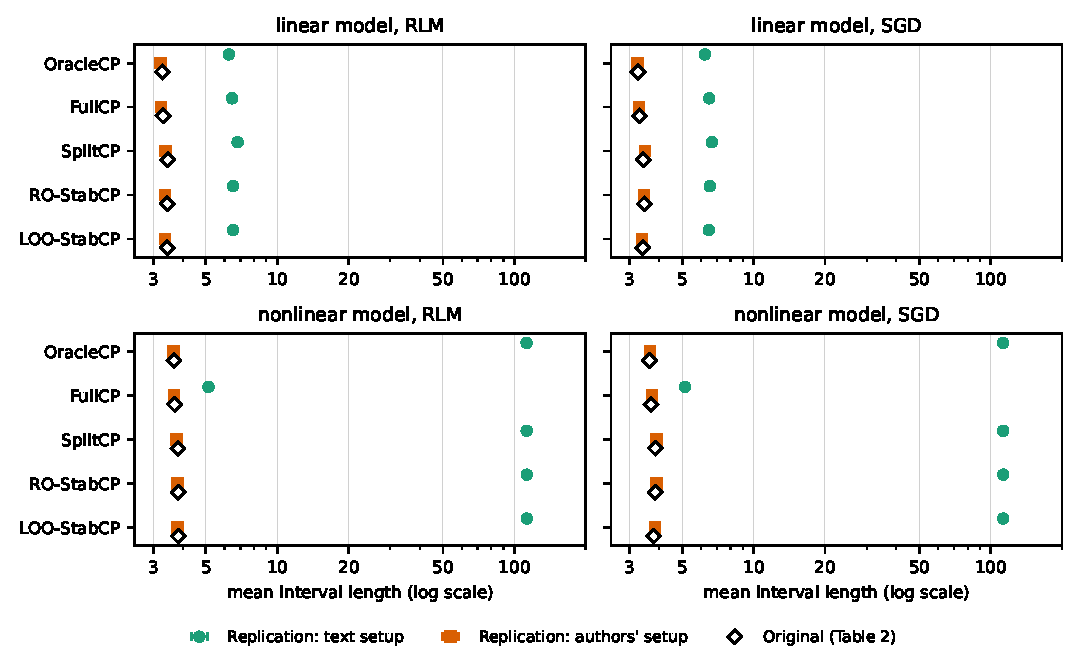
\includegraphics[width=\linewidth]{article_sim_setups.pdf}
\caption{Mean interval length on synthetic data, by method, under the text setup, under the authors' setup (with
$\pm2$ standard errors) and in Table~2 of the original. The horizontal axis is logarithmic. The authors' setup approaches
the original values; the text setup is offset by the change in the data-generating process (D1).}
\label{fig:sim}
\end{figure}

The gap under the text setup has a simple cause (D1). The text specifies $\|\beta\|^2=d$, so the signal $X^\top\beta$
has variance of order one and the optimal interval is wider than the $2\times1.645=3.29$ of pure noise. The
supplement's code uses the text's AR(1) design but $\|\beta\|^2=1/d$, so the signal variance is about $10^{-4}$, the
response is essentially noise, and the oracle length is close to 3.29, as in Table~2 of the original. The supplement's
result file for this design reproduces every cell of Table~2 exactly, which strongly supports this configuration as the source of the table; its provenance has not been confirmed with the authors. (The
later repository version also replaces the AR(1) design by independent features; with a signal this weak that changes
replication lengths by at most 0.002.) In the nonlinear model the
text's design gives $E[Y]=\sum_k\beta_k E[e^{X_k/10}]\approx55$, which a linear model without intercept cannot fit;
hence lengths near 113. When the response is centered on its training mean (a check run before the code was consulted), the
nonlinear RLM lengths fall to 3.2--3.4 (OracleCP 3.227, SplitCP 3.438, \LOO\ 3.393). Under the authors' design the
same offset is only about 0.55, which explains why their nonlinear lengths exceed their linear ones. The original's
FullCP rows are identical for RLM and SGD; this is consistent with the coarse grid of D6, which maps two near-zero
predictors to the same accepted range. In the repository's result file the per-repetition lengths of the two differ by at
most 0.002.

\paragraph{C1.} \LOO\ coverage lies between 0.901 and 0.908 in all eight runs of Table~\ref{tab:sim}; the SE is computed across the 100 repetition-level coverages, since test outcomes within a repetition share a fitted model. This is an empirical check of the coverage claim, not a proof of validity.
\textbf{Verdict: reproduced.}

\paragraph{C4.} For RLM, \LOO\ and \RO\ have the same length to within 0.001 under both setups. For SGD, \LOO\ is
shorter than \RO\ in all four comparisons: 6.475 vs 6.534 and 112.968 vs 113.028 under the text setup, 3.391 vs 3.451
and 3.829 vs 3.889 under the authors' setup, against 3.405 vs 3.464 and 3.789 vs 3.849 in the original.
\textbf{Verdict: reproduced.} C2 is assessed in Section~\ref{sec:c2}, after the real-data results.

\subsection{Coverage and length on real data (C1, C4)}

Table~\ref{tab:real} reports the real-data experiment with $m=100$ held-out points. The columns are as in
Table~\ref{tab:sim}, except that the original reports only coverage (Table~3 of the original); the last column gives
the mean length in the authors' published result file. Under the text setup RLM intervals are \emph{shorter} than the
authors', while SGD-based \RO\ and \LOO\ are conservative (coverage 0.958--0.990) and long. The authors' setup
removes both effects: its lengths are within 0.057 of the authors' file (19 of 20 rows within 0.025) and its
coverages within 0.017 of Table~3. Figure~\ref{fig:real} shows the lengths.

\begin{table}[htbp]
\centering\footnotesize\setlength{\tabcolsep}{4.5pt}
\caption{Real data, $m=100$ test points: mean coverage and length over 100 repetitions. ``Original'' coverage is
Table~3 of the original paper; ``Authors' file'' length is the mean length in the authors' published result file,
since the paper shows lengths only as box plots. Lengths are in units of the standard deviation of the response.}
\label{tab:real}
\begin{tabular}{@{}llrrrrrr@{}}
\toprule
& & \multicolumn{2}{c}{Text setup} & \multicolumn{2}{c}{Authors' setup} & Original & Authors' file \\
\cmidrule(lr){3-4}\cmidrule(lr){5-6}\cmidrule(lr){7-7}\cmidrule(l){8-8}
Data, model & Method & Coverage & Length & Coverage & Length & Coverage & Length \\
\midrule
Boston, RLM & OracleCP & 0.899 & 1.907 & 0.900 & 2.850 & 0.906 & 2.854 \\
 & FullCP & 0.898 & 1.944 & 0.889 & 2.782 & 0.897 & 2.807 \\
 & SplitCP & 0.902 & 2.017 & 0.895 & 2.861 & 0.898 & 2.860 \\
 & \RO & 0.920 & 2.195 & 0.900 & 2.870 & 0.905 & 2.874 \\
 & \LOO & 0.920 & 2.183 & 0.900 & 2.869 & 0.905 & 2.873 \\
\addlinespace
Boston, SGD & OracleCP & 0.893 & 1.448 & 0.895 & 1.757 & 0.905 & 1.776 \\
 & FullCP & 0.893 & 1.537 & 0.887 & 2.116 & 0.901 & 2.173 \\
 & SplitCP & 0.897 & 1.567 & 0.884 & 1.883 & 0.901 & 1.908 \\
 & \RO & 0.990 & 3.136 & 0.901 & 1.874 & 0.910 & 1.892 \\
 & \LOO & 0.961 & 2.284 & 0.897 & 1.815 & 0.906 & 1.833 \\
\addlinespace
Diabetes, RLM & OracleCP & 0.900 & 2.502 & 0.901 & 2.869 & 0.900 & 2.867 \\
 & FullCP & 0.899 & 2.530 & 0.884 & 2.809 & 0.889 & 2.824 \\
 & SplitCP & 0.902 & 2.540 & 0.889 & 2.852 & 0.894 & 2.872 \\
 & \RO & 0.935 & 2.732 & 0.901 & 2.889 & 0.900 & 2.888 \\
 & \LOO & 0.936 & 2.726 & 0.901 & 2.888 & 0.900 & 2.887 \\
\addlinespace
Diabetes, SGD & OracleCP & 0.907 & 2.326 & 0.906 & 2.409 & 0.902 & 2.403 \\
 & FullCP & 0.909 & 2.400 & 0.887 & 2.601 & 0.890 & 2.620 \\
 & SplitCP & 0.908 & 2.433 & 0.900 & 2.494 & 0.902 & 2.513 \\
 & \RO & 0.979 & 3.501 & 0.916 & 2.519 & 0.914 & 2.512 \\
 & \LOO & 0.958 & 2.924 & 0.909 & 2.464 & 0.906 & 2.457 \\
\bottomrule
\end{tabular}
\end{table}

\begin{figure}[htbp]
\centering
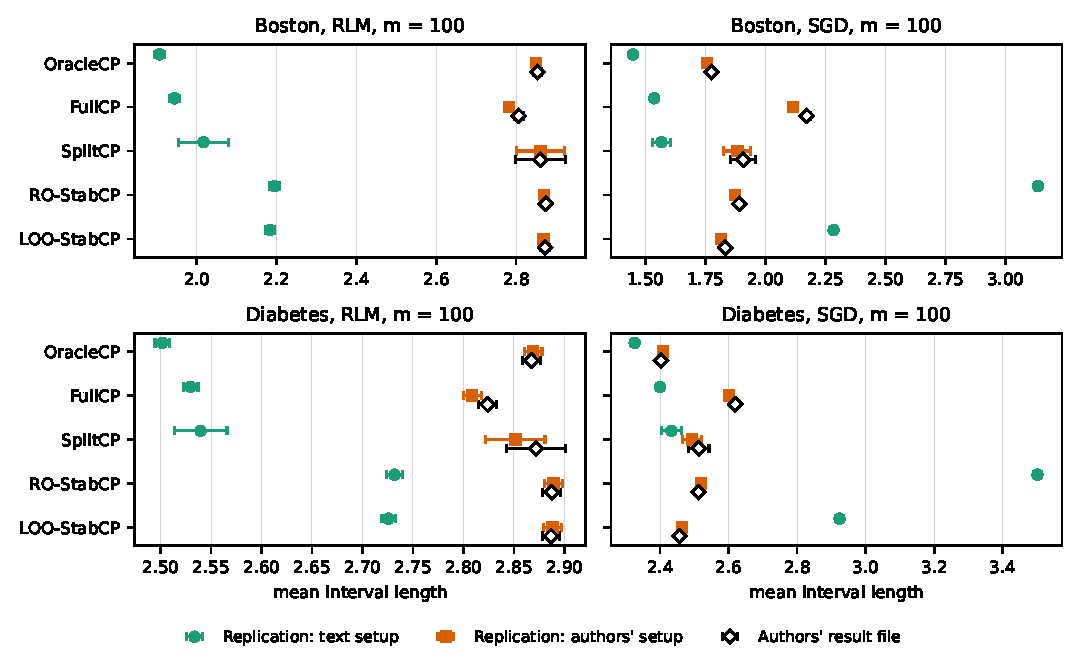
\includegraphics[width=\linewidth]{article_real_setups.pdf}
\caption{Mean interval length on real data ($m=100$), by method, under the text setup, under the authors' setup and
in the authors' published result file. Under the authors' setup replication values approach those in the authors' file; under
the text setup the SGD stability bounds are about ten times larger and \RO\ and \LOO\ become the longest methods.}
\label{fig:real}
\end{figure}

The cause is feature scaling (D2). The paper says only that continuous variables are ``normalized''. The authors'
code z-scores them and then divides by $\sqrt d$, so $\|X_i\|\approx1$ rather than $\approx\sqrt d$. With a fixed
penalty $\|\theta\|^2$ this strengthens the regularization $d$-fold, which explains why the text-setup RLM intervals
are shorter: the less regularized model fits better. The SGD bounds of Eq.~(\ref{eq:sgdbound}) are proportional to
$\|X_i\|\|X_{n+j}\|$ and therefore $d$ times larger under the text setup (13 times for Boston and 10 times for
Diabetes), which makes \RO\ and \LOO\ conservative. Appendix~\ref{app:real} decomposes the authors' setup into its
parts and shows that D2 alone accounts for nearly all of the change.

With $m=1$ the coverage of a repetition is 0 or 1, so the Monte-Carlo standard error of a mean coverage over 100
repetitions is about 0.03. The replication $m=1$ \LOO\ coverages range from 0.86 to 0.96 and those of the original from 0.90 to
0.92 (Appendix~\ref{app:real}). With the RLM bound computed with $\lambda=1$ instead of 2, \LOO\ coverage at $m=100$
rises from 0.920 to 0.933 (Boston) and from 0.936 to 0.959 (Diabetes), and the lengths from 2.183 to 2.444 and from
2.726 to 2.940.

\paragraph{C1.} \LOO\ coverage at $m=100$ is between 0.897 and 0.961 in all eight runs of Table~\ref{tab:real}. The
lowest value, 0.897, is 0.003 below the nominal level, smaller than its repetition-level SE (0.0029).
\textbf{Verdict: reproduced.}

\paragraph{C4.} \LOO\ is shorter than \RO\ for SGD in all four comparisons: 2.284 vs 3.136 (Boston) and 2.924 vs 3.501
(Diabetes) under the text setup, and 1.815 vs 1.874 and 2.464 vs 2.519 under the authors' setup. For RLM the two
differ by at most 0.012. \textbf{Verdict: reproduced.}

\subsection{Interval length relative to SplitCP (C2)}
\label{sec:c2}

Claim C2 has two parts: \LOO\ is competitive with the full-data methods, and SplitCP is longer and more variable.
Tables~\ref{tab:sim} and~\ref{tab:real} settle the first part. Under the authors' setup \LOO\ is at most 5\% longer
than OracleCP and at most 0.15 longer than FullCP in every row; for SGD on real data it is shorter than FullCP, which
is trained for only 5 epochs. Table~\ref{tab:c2} isolates the second part. For each setting it gives the mean and the
standard deviation (sd) over repetitions of the interval length of \LOO\ and SplitCP, and the difference of the means.
Negative differences favor \LOO. The final column gives the SE of the paired difference for replication runs, using the same data repetition for both methods. A small observed difference does not establish equivalence.

\begin{table}[htbp]
\centering\small
\caption{\LOO\ versus SplitCP: mean and standard deviation (sd) over repetitions of the interval length.
``Difference'' is the \LOO\ mean minus the SplitCP mean, computed before rounding; negative values favor \LOO.
Synthetic rows show the two replication setups and Table~2 of the original, which gives no \LOO\ sd for three settings (--).
Real-data rows ($m=100$) show the two replication setups and the authors' result file. SE(diff.) is the SD of the paired length differences divided by $\sqrt{100}$ for replication runs; -- means it is not reported here for the original results.}
\label{tab:c2}
\begin{tabular}{@{}lrrrrrr@{}}
\toprule
& \multicolumn{3}{c}{Mean length} & \multicolumn{2}{c}{SD of length} & \\
\cmidrule(lr){2-4}\cmidrule(l){5-6}
Source & \LOO & SplitCP & Difference & \LOO & SplitCP & SE(diff.) \\
\midrule
\multicolumn{7}{@{}l}{\emph{Synthetic, linear, RLM}} \\
\quad Text setup & 6.515 & 6.808 & $-0.293$ & 0.548 & 1.073 & 0.097 \\
\quad Authors' setup & 3.371 & 3.373 & $-0.002$ & 0.296 & 0.542 & 0.045 \\
\quad Original & 3.442 & 3.455 & $-0.013$ & 0.257 & 0.514 & -- \\
\addlinespace
\multicolumn{7}{@{}l}{\emph{Synthetic, linear, SGD}} \\
\quad Text setup & 6.475 & 6.670 & $-0.195$ & 0.537 & 1.085 & 0.098 \\
\quad Authors' setup & 3.391 & 3.488 & $-0.097$ & 0.325 & 0.541 & 0.049 \\
\quad Original & 3.405 & 3.420 & $-0.015$ & -- & 0.557 & -- \\
\addlinespace
\multicolumn{7}{@{}l}{\emph{Synthetic, nonlinear, RLM}} \\
\quad Text setup & 112.970 & 112.906 & $+0.064$ & 0.336 & 0.589 & 0.051 \\
\quad Authors' setup & 3.805 & 3.764 & $+0.040$ & 0.307 & 0.584 & 0.056 \\
\quad Original & 3.827 & 3.812 & $+0.015$ & -- & 0.554 & -- \\
\addlinespace
\multicolumn{7}{@{}l}{\emph{Synthetic, nonlinear, SGD}} \\
\quad Text setup & 112.968 & 113.031 & $-0.062$ & 0.342 & 0.681 & 0.063 \\
\quad Authors' setup & 3.829 & 3.887 & $-0.058$ & 0.344 & 0.570 & 0.046 \\
\quad Original & 3.789 & 3.855 & $-0.066$ & -- & 0.612 & -- \\
\addlinespace
\multicolumn{7}{@{}l}{\emph{Boston, RLM}} \\
\quad Text setup & 2.183 & 2.017 & $+0.167$ & 0.058 & 0.317 & 0.032 \\
\quad Authors' setup & 2.869 & 2.861 & $+0.008$ & 0.058 & 0.299 & 0.030 \\
\quad Authors' file & 2.873 & 2.860 & $+0.013$ & 0.053 & 0.310 & -- \\
\addlinespace
\multicolumn{7}{@{}l}{\emph{Boston, SGD}} \\
\quad Text setup & 2.284 & 1.567 & $+0.718$ & 0.054 & 0.187 & 0.019 \\
\quad Authors' setup & 1.815 & 1.883 & $-0.068$ & 0.058 & 0.281 & 0.028 \\
\quad Authors' file & 1.833 & 1.908 & $-0.075$ & 0.064 & 0.264 & -- \\
\addlinespace
\multicolumn{7}{@{}l}{\emph{Diabetes, RLM}} \\
\quad Text setup & 2.726 & 2.540 & $+0.186$ & 0.037 & 0.131 & 0.013 \\
\quad Authors' setup & 2.888 & 2.852 & $+0.037$ & 0.045 & 0.146 & 0.014 \\
\quad Authors' file & 2.887 & 2.872 & $+0.015$ & 0.044 & 0.144 & -- \\
\addlinespace
\multicolumn{7}{@{}l}{\emph{Diabetes, SGD}} \\
\quad Text setup & 2.924 & 2.433 & $+0.491$ & 0.054 & 0.145 & 0.015 \\
\quad Authors' setup & 2.464 & 2.494 & $-0.030$ & 0.041 & 0.135 & 0.013 \\
\quad Authors' file & 2.457 & 2.513 & $-0.056$ & 0.038 & 0.152 & -- \\
\bottomrule
\end{tabular}
\end{table}

Three patterns stand out. First, the reported SD of \LOO\ length is smaller than SplitCP's in every row where both are available. Second, under the authors' setup \LOO\ has a smaller mean length for SGD in all four settings, by 0.030--0.097. Third, for RLM the authors'-setup differences are $-0.002$, $+0.040$, $+0.008$ and $+0.037$, so \LOO\ is longer in three of the four settings. Their paired SEs are 0.045, 0.056, 0.030 and 0.014, respectively. These are descriptive comparisons: they do not show that the RLM methods have equal expected length. Under the text setup on real data, \LOO\ is longer than SplitCP for both models. Thus the shorter-interval claim depends on the model and, on real data, on feature scaling.

\paragraph{C2.} \textbf{Verdict: partially reproduced.} \LOO\ is competitive with OracleCP, FullCP and \RO, and is
consistently less variable than SplitCP. It is shorter on average than SplitCP for SGD under the authors' setup, but
not for RLM, and not on real data under the text setup.

\subsection{Run time (C3)}

Table~\ref{tab:time} reports the mean wall-clock time per repetition ($m=100$ test points) in the linear synthetic
setting under the text setup, together with the times in Table~2 of the original. The ratio columns divide each
method's time by \LOO's time in the same source, which permits a within-source comparison but does not remove solver or hardware effects on relative costs.

\begin{table}[htbp]
\centering\small
\caption{Mean time per repetition in seconds, linear synthetic setting, $m=100$. ``Replication'' is the text setup;
``Original'' is Table~2 of the original paper. ``Ratio to \LOO'' divides each time by the \LOO\ time of the same
source and model, using unrounded times.}
\label{tab:time}
\begin{tabular}{@{}llrrrr@{}}
\toprule
& & \multicolumn{2}{c}{Time (s)} & \multicolumn{2}{c}{Ratio to \LOO} \\
\cmidrule(lr){3-4}\cmidrule(l){5-6}
Model & Method & Replication & Original & Replication & Original \\
\midrule
RLM & OracleCP & 0.0178 & 3.201 & 24.6 & 91.5 \\
 & FullCP & 0.4935 & 176.783 & 681.3 & 5050.9 \\
 & SplitCP & 0.0003 & 0.017 & 0.3 & 0.5 \\
 & \RO & 0.0178 & 3.190 & 24.6 & 91.1 \\
 & \LOO & 0.0007 & 0.035 & 1.0 & 1.0 \\
\addlinespace
SGD & OracleCP & 0.0254 & 0.720 & 47.1 & 80.0 \\
 & FullCP & 0.6282 & 19.320 & 1161.6 & 2146.7 \\
 & SplitCP & 0.0002 & 0.005 & 0.4 & 0.6 \\
 & \RO & 0.0176 & 0.720 & 32.5 & 80.0 \\
 & \LOO & 0.0005 & 0.009 & 1.0 & 1.0 \\
\bottomrule
\end{tabular}
\end{table}

The ordering SplitCP $<$ \LOO\ $\ll$ \RO\ $\approx$ OracleCP $\ll$ FullCP is the same in both sources. Replication absolute
times are 17 to 358 times shorter, mainly because the replication solves RLM by Newton's method instead of a general convex solver
(D8). The speed-ups of \LOO\ over \RO\ (25 and 32 times) are correspondingly smaller than the original's (91 and 80
times), because the fixed cost of computing bounds weighs more when fits are cheap. On real data the gap grows with
$m$ as claimed: for Boston RLM under the text setup, \RO\ and \LOO\ take 0.00027~s and 0.00024~s at $m=1$, and
0.0104~s and 0.00086~s at $m=100$ (12 times). For neural networks under the authors' setup, \LOO\ takes 0.011--0.016~s
per repetition and \RO\ 0.97--1.45~s (Section~\ref{sec:nn}).

\paragraph{C3.} \textbf{Verdict: reproduced.} The ordering and the growth with $m$ hold; the size of the speed-up
depends on the cost of a single fit and is smaller in this implementation.

\subsection{Neural networks (C5)}
\label{sec:nn}

The original reports the neural-network results only as box plots: Fig.~3 (one hidden layer of 20 units) and Fig.~6
(hidden layers of 10 and 5 units). The supplement's \texttt{results\_nn.csv} holds the raw coverage, length and time of
one run, 100 repetitions per data set and method, without a column for the architecture. Its medians agree with the
medians previously digitized from Fig.~6 to within 0.006, and differ from those of Fig.~3 by 0.24--0.80, so it is the
two-layer run, although the shipped \texttt{real\_NN.py} is set to one layer of 20 units (D20). The two-layer comparison therefore uses the raw file; the one-layer comparison uses only digitized medians (Appendix~\ref{app:digitise}).

The supplement's network differs from the one the text describes in three ways: ReLU instead of sigmoid units (D17),
scikit-learn's \texttt{MLPRegressor} with squared loss, mini-batches, momentum, weight decay, early stopping and the
same random initialization for every fit (D18), and a constant stability bound $R\eta$ instead of Eq.~(8) (D19).
Table~\ref{tab:nn} switches these on one group at a time, starting from the text setup.

\begin{table}[htbp]
\centering\footnotesize\setlength{\tabcolsep}{3.5pt}
\caption{Neural networks on real data ($m=100$): mean interval length over 100 repetitions under five versions of the
experiment, and mean coverage under the authors' setup. ``D2--D7'' is the text setup with the repository's data and
conformal choices but the initial network; ``+ network'' adds the supplement's network (D17, D18); ``Authors''' adds its
constant bound (D19). ``File'' is the supplement's \texttt{results\_nn.csv}, which exists only for two hidden layers
(--).}
\label{tab:nn}
\begin{tabular}{@{}lllrrrrrrr@{}}
\toprule
& & & \multicolumn{5}{c}{Mean length} & \multicolumn{2}{c}{Mean coverage} \\
\cmidrule(lr){4-8}\cmidrule(l){9-10}
Hidden & Data & Method & Text & D2--D7 & + network & Authors' & File & Authors' & File \\
\midrule
% generated by scripts/compare_supplement.py from results/raw/nn*.csv and results_nn.csv
\inputtable{tables/nn.tex}
\bottomrule
\end{tabular}
\end{table}

\begin{figure}[htbp]
\centering
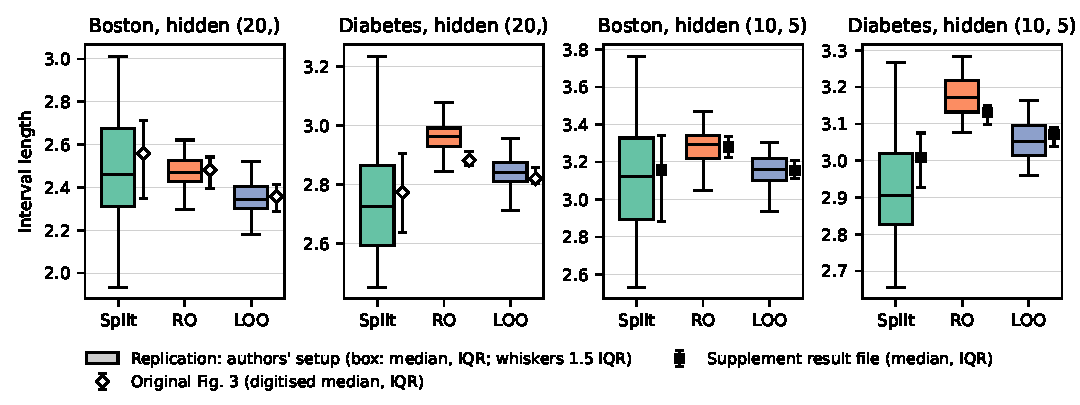
\includegraphics[width=\linewidth]{article_nn.pdf}
\caption{Interval length of the neural networks under the authors' setup (box plots over 100 repetitions). Filled
squares: median and interquartile range of the supplement's raw result file (two hidden layers). Open diamonds:
median and interquartile range digitized from Fig.~3 of the original (one hidden layer), for which no raw file
was found in the inspected materials.}
\label{fig:nn}
\end{figure}

Under the text setup the heuristic bounds are $d$ times larger, for the reason given in Section~\ref{sec:results}
(D2), so \RO\ (coverage 0.994--1.000) and \LOO\ (0.961--0.985) are very conservative and their intervals are the
longest. Feature scaling removes most of the gap, and the supplement's network removes the rest: under the authors'
setup the two-layer mean lengths are within 0.085 of the raw file and the \LOO\ rows within 0.003; the one-layer
medians are within 0.10 of the digitized ones (Boston SplitCP 2.461 vs 2.558, all others within 0.081). The network
matters mostly for Diabetes, where \LOO\ falls from 3.254 to 3.050 (file 3.059). The constant bound changes lengths
by at most 0.034, because with $\|X_i\|\approx1$ it has the same size as Eq.~(8). Coverage under the authors' setup is
0.904--0.914 for \LOO, 0.914--0.940 for \RO\ and 0.887--0.895 for SplitCP; the file has 0.889--0.915.

\LOO\ is shorter than \RO\ in every panel, in every source. The comparison with SplitCP is mixed, and now in the same
way as in the original: \LOO\ is clearly shorter only for Boston with one layer (median 2.342 vs 2.461; digitized 2.358
vs 2.558), about tied for Boston with two layers (mean 3.151 vs 3.141; file 3.151 vs 3.119) and longer for Diabetes
with either architecture. Under the authors' setup \LOO\ takes 0.011--0.016~s per repetition and \RO\ 0.97--1.45~s,
85 to 91 times as long (file: 0.006--0.011~s and 0.33--0.84~s).

\paragraph{C5.} \textbf{Verdict: reproduced with qualification.} \LOO\ has empirical coverage near or above 0.9 for the tested neural networks and is 85--91 times faster than \RO\ under the authors' setup. Numerical agreement is strongest for the two-layer \LOO\ rows, but only with the unreported feature
scaling and with a network and bound that differ from the paper's description. Its intervals are comparable to
SplitCP's, not uniformly shorter. With features scaled as in the text setup, its observed coverage is conservative. The heuristic bound does not itself establish a general validity guarantee for these networks.

\subsection{Kernels (C6)}
\label{sec:kernel}

App.~A.1 of the original repeats the synthetic experiment of §4 with an RBF kernel ($\sigma=0.1$) and a polynomial
kernel of degree 2, and reports in Fig.~5 that coverage is kept and that the intervals are shorter in the nonlinear
setting. The paper does not say how the kernel enters the model or the stability bounds. Following the supplement's
\texttt{kernel.py}, each point is represented by its row of kernel values with the $n$ training points as centers, so
that the model is linear in $n$ features, and apply the ordinary SGD bound to these features. The supplement differs
from the text in two parameters (D21, D22): it sets the RBF kernel to $\exp(-0.1\|x-x'\|^2)$, i.e.\ $\sigma\approx2.24$
rather than 0.1, and the SGD step size to $\eta=10^{-5}$ with a kernel ($10^{-3}$ without). It runs SGD only. Table~\ref{tab:kernel}
compares replication runs with the supplement's \texttt{results\_kernel.csv}.

\begin{table}[htbp]
\centering\footnotesize\setlength{\tabcolsep}{3.5pt}
\caption{Kernels (SGD, $n=m=100$, $d=100$): mean coverage and mean length over 100 repetitions. ``Text'' uses the
text's design and $\sigma=0.1$ with $\eta=0.001$; ``Authors''' uses the supplement's design (D1) and kernel
parameters (D21, D22); ``File'' is the supplement's \texttt{results\_kernel.csv}; ``Centered'' is the authors' setup
with the response centered at its training mean. Cov. denotes empirical coverage. The no-kernel rows are separately seeded kernel-experiment runs, not reused rows of Table~\ref{tab:sim}; consequently their means differ even when their settings coincide.}
\label{tab:kernel}
\begin{tabular}{@{}lllrrrrrrrr@{}}
\toprule
& & & \multicolumn{2}{c}{Text} & \multicolumn{2}{c}{Authors'} & \multicolumn{2}{c}{File} & \multicolumn{2}{c}{Centered} \\
\cmidrule(lr){4-5}\cmidrule(lr){6-7}\cmidrule(lr){8-9}\cmidrule(l){10-11}
Setting & Kernel & Method & Cov. & Length & Cov. & Length & Cov. & Length & Cov. & Length \\
\midrule
% generated by scripts/compare_supplement.py from results/raw/kernel*.csv and results_kernel.csv
\inputtable{tables/kernel.tex}
\bottomrule
\end{tabular}
\end{table}

Under the authors' setup replication results match the file: every mean length is within 0.102 and every coverage within
0.013. The observed coverages range from 0.893 to 0.912, and in the nonlinear setting both kernels shorten \LOO\ from 3.859
to 3.475 (RBF) and 3.464 (polynomial); the file has 3.849, 3.487 and 3.413. In the linear setting the kernels do not
help (3.327 without, 3.378 and 3.347 with). \LOO\ is again far less variable than SplitCP (sd of length 0.29--0.37 vs
0.50--0.67).

A response-centering check supports an offset-based explanation for the gain. Both kernel maps contain a large, almost constant component: with $\gamma=0.1$ and
$\|X_i-X_j\|^2\approx2$ every RBF entry is about $e^{-0.2}\approx0.82$, and the polynomial kernel adds 1. This
component acts as an intercept, which the no-kernel model lacks, and absorbs the offset $\sum_k\beta_k\approx0.55$ of
the nonlinear response (Section~\ref{sec:results}). When the response is centered, the advantage disappears: nonlinear
\LOO\ lengths are 3.367 without a kernel, 3.358 with the RBF kernel and 3.405 with the polynomial kernel.

With the text's parameters the experiment does not work. With $\sigma=0.1$ the off-diagonal RBF entries are about
$e^{-100}$, so the features carry no information about test points and the lengths are close to those without a
kernel (about 113 in the nonlinear setting). The polynomial features have norms near 10, and with $\eta=0.001$ the SGD bounds
dominate: \LOO\ covers 1.000 (linear) and 0.996 (nonlinear) with lengths 11.575 and 12.181, while SplitCP under-covers
(0.883 and 0.784). A possible explanation for the under-coverage is that a calibration point is itself one of the kernel centers,
so its feature vector contains its own kernel value $k(x_i,x_i)$ and a test point's does not, but this explanation was not tested. Kernel RLM with penalty $\theta^\top K\theta$, which App.~A.1 describes but the supplement does not run, behaves
in the same way (polynomial \LOO\ coverage 1.000, length 21.747 linear; RBF as without a kernel). The supplement's
kernel parameters alone, on the text's design, give lengths of 6.5--6.7 (linear) and 109.8--111.7 (nonlinear), with
coverage 0.897--0.910 among the kernel rows (excluding the no-kernel baseline).

\paragraph{C6.} \textbf{Verdict: reproduced with qualification.} Kernel SGD keeps coverage and gives shorter intervals
in the nonlinear setting, as claimed, and the replication values match the authors' raw results. But this depends on a bandwidth that differs from the stated value and a
step size that the paper does not report (with the stated $\sigma=0.1$ the RBF kernel is degenerate), and the centering experiment indicates that the gain in this design is largely attributable to the offset handled by the kernel features. It does not establish a general limitation of kernel methods.

\subsection{Derandomized split conformal (C7)}

Table~\ref{tab:derand} compares \LOO\ with MM-SplitCP and EM-SplitCP under the two replication setups and in the supplement's
result files, which hold the raw numbers behind Figs.~7 and~8 of the original. In the authors' setup each of the $K$
split intervals is computed at level $1-\alpha/2$ with the code's quantile rule (D5), and $K=50$ on real data as in
the supplement (D10); the text setup uses $K=30$ and the text's quantile rule throughout.

\begin{table}[htbp]
\centering\footnotesize
\caption{\LOO\ versus derandomized split conformal, $m=100$, 100 repetitions: mean coverage (Cov.) and mean interval
length. ``Supplement file'' is \texttt{results\_synthetic\_derandom.csv} ($K=30$) or \texttt{results\_real\_derandom.csv}
($K=50$) from the authors' supplementary material.}
\label{tab:derand}
\begin{tabular}{@{}llrrrrrr@{}}
\toprule
& & \multicolumn{2}{c}{\LOO} & \multicolumn{2}{c}{MM-SplitCP} & \multicolumn{2}{c}{EM-SplitCP} \\
\cmidrule(lr){3-4}\cmidrule(lr){5-6}\cmidrule(l){7-8}
Data, model & Source & Cov. & Length & Cov. & Length & Cov. & Length \\
\midrule
% generated by scripts/compare_supplement.py from results/raw/{sim,real}{,_authors}.csv and the supplement files
\inputtable{tables/derand.tex}
\bottomrule
\end{tabular}
\end{table}

Under the authors' setup, every coverage in Table~\ref{tab:derand} differs from the supplement files by at most 0.011 and every length by at most 0.115. Both derandomized methods have mean coverage above 0.9 (0.904--0.946 in replication runs), and their mean lengths are 1.02--1.62 times \LOO's (files: 1.02--1.63). Their measured computation times are 4.5--8.4 times \LOO's in these runs (files: 18--197 times), consistent with the additional cost of fitting $K$ models.

The length comparison is not invariant to the setup. Under the text setup the synthetic rows and real-data RLM rows favor \LOO, but both real-data SGD rows favor the derandomized methods. On Boston, \LOO\ has mean length 2.284, compared with 2.155 for MM-SplitCP and 1.926 for EM-SplitCP; on Diabetes the corresponding values are 2.924, 2.776 and 2.612. All three methods have mean coverage above 0.9 in those rows. On Boston both derandomized methods cover less often than \LOO; on Diabetes MM-SplitCP covers 0.959 versus 0.958 for \LOO, while EM-SplitCP covers 0.939. Thus the speed advantage is more robust than the length advantage.

\paragraph{C7.} \textbf{Verdict: partially reproduced.} \LOO\ is faster in the reported comparisons and shorter than both baselines under the authors' setup and in the supplement files, but not for real-data SGD under the text setup.

\subsection{Conformal screening (C8)}

Tables~\ref{tab:power} and~\ref{tab:fdr} report the screening experiment. Each table has one row per FDR level $q$ and
method, and four columns: the text setup, the authors' setup, the authors' setup with the LOO-cfBH bound corrected
(D14; everything else unchanged), and Table~4 of the original. Power carries the claim, so it is discussed first.
Figure~\ref{fig:screen} shows the same data.

\begin{table}[htbp]
\centering\small
\caption{Screening: mean power over 1000 repetitions. ``Authors', bound corrected'' restores the factor $R$ missing
from the LOO-cfBH training-point bound in the authors' code; it changes only the LOO-cfBH rows. ``Original'' is
Table~4 of the original paper. Under the authors' setup only 10 distinct train/test splits are used (D12), so the
standard error of a LOO-cfBH power value is about 0.035 at $q=0.1$, 0.011 at $q=0.2$ and 0.002 at $q=0.3$.}
\label{tab:power}
\begin{tabular}{@{}llrrrr@{}}
\toprule
$q$ & Method & Text setup & Authors' setup & Authors', bound corrected & Original \\
\midrule
0.1 & cfBH & 0.660 & 0.628 & 0.628 & 0.632 \\
 & RO-cfBH & 0.000 & 0.286 & 0.286 & 0.304 \\
 & LOO-cfBH & 0.185 & 0.608 & 0.483 & 0.674 \\
\addlinespace
0.2 & cfBH & 0.921 & 0.938 & 0.938 & 0.928 \\
 & RO-cfBH & 0.002 & 0.628 & 0.628 & 0.652 \\
 & LOO-cfBH & 0.725 & 0.965 & 0.896 & 0.943 \\
\addlinespace
0.3 & cfBH & 0.987 & 0.997 & 0.997 & 0.992 \\
 & RO-cfBH & 0.208 & 0.980 & 0.980 & 0.963 \\
 & LOO-cfBH & 0.943 & 0.998 & 0.998 & 0.992 \\
\bottomrule
\end{tabular}
\end{table}

\begin{table}[htbp]
\centering\small
\caption{Screening: false discovery rate, the mean false discovery proportion over 1000 repetitions. Columns as in
Table~\ref{tab:power}. The target is $q$.}
\label{tab:fdr}
\begin{tabular}{@{}llrrrr@{}}
\toprule
$q$ & Method & Text setup & Authors' setup & Authors', bound corrected & Original \\
\midrule
0.1 & cfBH & 0.088 & 0.087 & 0.087 & 0.093 \\
 & RO-cfBH & 0.000 & 0.011 & 0.011 & 0.004 \\
 & LOO-cfBH & 0.006 & 0.048 & 0.035 & 0.066 \\
\addlinespace
0.2 & cfBH & 0.189 & 0.207 & 0.207 & 0.200 \\
 & RO-cfBH & 0.000 & 0.066 & 0.066 & 0.060 \\
 & LOO-cfBH & 0.077 & 0.195 & 0.158 & 0.184 \\
\addlinespace
0.3 & cfBH & 0.280 & 0.295 & 0.295 & 0.288 \\
 & RO-cfBH & 0.064 & 0.228 & 0.228 & 0.248 \\
 & LOO-cfBH & 0.199 & 0.289 & 0.274 & 0.284 \\
\bottomrule
\end{tabular}
\end{table}

\begin{figure}[htbp]
\centering
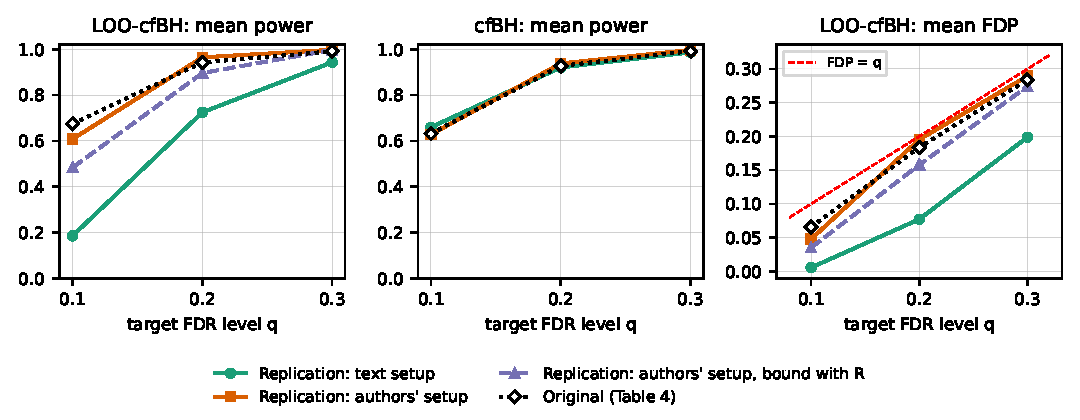
\includegraphics[width=\linewidth]{article_screening.pdf}
\caption{Screening results against the FDR level $q$: LOO-cfBH power, cfBH power, and LOO-cfBH false discovery rate
with the line FDR $=q$. Lines show the text setup, the authors' setup, the authors' setup with the corrected bound,
and Table~4 of the original.}
\label{fig:screen}
\end{figure}

\paragraph{Power.} cfBH, which needs no stability bound, matches the original under both setups (within 0.03). Under
the text setup LOO-cfBH and RO-cfBH have far less power than in the original (LOO-cfBH 0.185 against 0.674 at
$q=0.1$). The main cause is feature scaling (D13), the screening analogue of D2: with the regression set-up of §5 the
features have norms of 3 to 5, and the bounds, which scale with $\|X_i\|\|X_{n+j}\|$, are large compared with
predictions in $[0,1]$. Applying only the authors' scaling raises LOO-cfBH power at $q=0.1$ from 0.185 to 0.602, and
RO-cfBH power from 0.000 to 0.473 (Appendix~\ref{app:screen}). The authors' setup then comes close to the original: every
power value is within 0.025 of Table~4, except LOO-cfBH at $q=0.1$ (0.608 against 0.674; absolute difference 0.066).

Under the authors' setup, LOO-cfBH is more powerful than cfBH only at $q=0.2$ (0.965 against 0.938); at $q=0.1$ it is
less powerful (0.608 against 0.628) and at $q=0.3$ their mean powers differ by only 0.001. With a fresh split in every repetition instead of
10 distinct splits, LOO-cfBH is ahead at $q=0.1$ (0.654 against 0.645) and $q=0.2$ (0.946 against 0.931). All of these runs, however, use the authors' training-point bound for LOO-cfBH, which
lacks the factor $R=15$ (D14; Section~\ref{sec:discussion}). With the bound as stated in the paper, LOO-cfBH power
falls to 0.483, 0.896 and 0.998, below cfBH at $q=0.1$ and $q=0.2$. LOO-cfBH is more powerful than RO-cfBH in every
setup and at every level, and is 10 (authors' setup) to 17 (text setup) times faster; the original reports 50 times
(0.0060~s against 0.2976~s).

\paragraph{FDR.} The mean FDP of LOO-cfBH and RO-cfBH is below $q$ in every setup and at every level, including with
the corrected bound. These are empirical estimates of expected FDP, not a finite-run proof of FDR control and not a guarantee about each repetition. cfBH slightly exceeds its target at $q=0.2$ under the authors' setup (0.207). The ten-split design limits the precision of this estimate, so this finite-run exceedance alone neither establishes nor refutes FDR control.

\paragraph{C8.} \textbf{Verdict: partially reproduced.} Observed mean FDPs are below the target levels, and the power and speed advantages over RO-cfBH are reproduced in the tested runs. The power advantage over cfBH is not: it appears only at $q=0.2$ in the authors' setup, and
it disappears when the stability bound is computed as stated in the paper.

\section{Discussion}
\label{sec:discussion}

\begin{table}[htbp]
\centering\small
\caption{Summary of verdicts. ``Depends on'' lists the differences from Table~\ref{tab:diffs} without which the
original numbers or the stated comparison are not obtained.}
\label{tab:verdicts}
\begin{tabular}{@{}l >{\raggedright\arraybackslash}p{4.8cm} >{\raggedright\arraybackslash}p{3.2cm} >{\raggedright\arraybackslash}p{3.2cm}@{}}
\toprule
Claim & Statement (abridged) & Verdict & Depends on \\
\midrule
C1 & Coverage at least $1-\alpha$ (empirical check) & Reproduced & -- \\
C2 & Competitive length; SplitCP longer and more variable & Partially reproduced & D1, D2 for the numbers \\
C3 & Speed on par with SplitCP, far below \RO\ and FullCP & Reproduced & -- \\
C4 & SGD: \LOO\ shorter than \RO & Reproduced & -- \\
C5 & Neural-network coverage and competitive length & Reproduced with qualification & D2; D17--D19 for the numbers \\
C6 & Kernels keep coverage, shorter nonlinear intervals & Reproduced with qualification & D1, D21, D22 \\
C7 & Less conservative and faster than MM- and EM-SplitCP & Partially reproduced & D1, D2, D5, D10 for the numbers \\
C8 & LOO-cfBH controls the FDR and is more powerful than cfBH & Partially reproduced & D13, D14 \\
\bottomrule
\end{tabular}
\end{table}

Table~\ref{tab:verdicts} separates the components of this partial replication. The empirical coverage and runtime results for the linear models broadly support C1 and C3, and the SGD interval comparison with \RO\ supports C4. The comparative-efficiency claims are less general: C2, C7 and C8 hold only in part, while C5 and C6 require qualifications about settings recovered from code. Agreement with a published table is distinct from reproducing its scientific interpretation. In particular, matching the screening implementation also reproduces a bound that differs from the stated method.

\paragraph{What the supplementary material changed.} The initial diagnosis used the public repository,
which covers only the synthetic, real-data and screening experiments. The ICLR supplement, consulted afterward,
contains code for the experiment families and raw results for all except the one-layer neural-network figure. It confirmed the two main diagnoses and corrected one detail: the
synthetic design that produced Table~2 keeps the text's correlated features and differs only in the scale of $\beta$
(D1). It also resolved questions left open in the initial diagnosis. The remaining neural-network differences come from the network the
code trains, which is not the one the paper describes (D17, D18); the derandomized baselines use the code's quantile
rule (D5) and, on real data, 50 rather than 30 splits (D10); and the kernel experiment uses a bandwidth different from the stated value and an unreported step
size (D21, D22). These choices substantially reduce the numerical differences, but do not make all comparisons indistinguishable at the scale of sampling error. For example, two-layer Diabetes SplitCP has mean length 2.922 in the replication run and 3.007 in the supplement, and Boston SGD FullCP has 2.116 versus 2.173 in the repository. The comparison therefore reports numerical gaps rather than claiming blanket agreement within Monte-Carlo error. The screening code and its result file in the supplement are identical to those in
the repository, including the bound discussed below.

\paragraph{Why the text does not reproduce the numbers.} Two data-preparation differences account for the largest
gaps in the linear regression experiments examined here. The synthetic data in the code differ from the description in the paper
(D1): the response is almost pure noise, so all methods have nearly the oracle length of 3.29. This changes the strength of signal being tested, so Table~2 of the original says little about a setting in which the features carry
signal. The real-data features are divided by $\sqrt d$ after standardization (D2). This is a substantive modeling
choice, not a detail: it multiplies the effective ridge penalty by $d$ and divides the SGD and neural-network
stability bounds by $d$. Under the literal reading, the SGD bounds dominate the interval width, and \LOO\ becomes
conservative and longer than SplitCP. The good performance of \LOO\ with SGD on real data therefore relies on features
of norm about one. In hindsight this is a natural choice, since the bounds scale with $\|X_i\|\|X_{n+j}\|$, but a
reader cannot infer it from the text.

\paragraph{A bug in the screening bound.} In the authors' screening code\supercite{authorscode}, the training-point
bound of LOO-cfBH is computed in \texttt{funcs/CP\_screening.py}, line 122, at commit \texttt{3b37682}, as
$\eta\gamma\nu_i\rho_{n+j}$, without the factor $R$ of the SGD bound in App.~G.1 (Eq.~(\ref{eq:sgdbound})). The
test-point bound on the next line, the RO-cfBH bound and the regression code all include $R$. The training-point
bounds used for LOO-cfBH in Table~4 of the original are therefore 15 times too small, and the resulting p-values are
not the p-values of Eq.~(\ref{eq:loop}) covered by the paper's FDR guarantee. In replication runs the mean FDP remained below the target levels, but the reported power advantage over cfBH depends on the smaller bound.

\paragraph{Ten distinct splits.} The authors' screening script redraws the train/test split only every hundredth
repetition, so its 1000 repetitions use 10 distinct splits (D12). The means move by less than 0.05 when every
repetition gets a fresh split, but the repetitions are not independent, and the effective number of replications for
split-dependent quantities is 10, not 1000. For LOO-cfBH power, the standard error computed from the 10 per-split
means is 0.035, 0.011 and 0.002 at the three levels, against a naive $\mathrm{sd}/\sqrt{1000}$ of 0.003, 0.001 and
0.0002. This uncertainty cautions against interpreting small power differences as robust advantages. Establishing uncertainty for a difference between methods would additionally require their split-level paired differences.

\paragraph{Diagnostic variants.} Table~\ref{tab:tried} lists the variants evaluated to locate the causes, roughly in the order
in which they were run. All except the first two were added after reading the authors' code.

\begin{table}[htbp]
\centering\small
\caption{Variants run to diagnose differences, with the main result of each. All numbers are replication means over 100
(regression) or 1000 (screening) repetitions.}
\label{tab:tried}
\begin{tabular}{@{}>{\raggedright\arraybackslash}p{4.4cm} >{\raggedright\arraybackslash}p{8.6cm}@{}}
\toprule
Variant & Main result \\
\midrule
RLM bound with $\lambda=1$ (text setup) & Bounds double; Boston \LOO\ coverage 0.920 $\to$ 0.933, length 2.183 $\to$
  2.444. Not a cause: the authors use $\lambda=2$ \\
Centered response (text setup, nonlinear) & Nonlinear RLM lengths fall from about 113 to 3.2--3.4 \\
Authors' setup with supplement design (D1) & Synthetic lengths within 2.4\% of Table~2 of the original \\
Real features divided by $\sqrt d$ (D2) & Real-data lengths close to the authors' file; SGD coverage back to about
  0.90 \\
Repository instead of supplement design (independent features) & Synthetic lengths change by at most 0.002 \\
Supplement network (D17, D18) & Diabetes two-layer \LOO\ length 3.254 $\to$ 3.050 (file 3.059) \\
Constant NN bound (D19) & Lengths change by at most 0.034 \\
$K=50$ on real data (D10) & MM/EM lengths change by at most 0.085 \\
Supplement kernel parameters (D21, D22) & Linear polynomial \LOO\ coverage 1.000 $\to$ 0.900, length 11.575 $\to$
  6.541 \\
Kernels with centered response & Nonlinear kernel gain disappears (\LOO\ 3.367 none, 3.358 RBF, 3.405 poly) \\
Shared SGD shuffles (D3) & No change at the third decimal \\
Authors' conformal details (D4--D7) & Length changes of up to 0.1; FullCP under-covers slightly, as in the original \\
Screening: authors' feature scaling (D13) & LOO-cfBH power at $q=0.1$: 0.185 $\to$ 0.602 \\
Screening: authors' LOO-cfBH bound (D14) & LOO-cfBH power at $q=0.1$: 0.185 $\to$ 0.549 \\
Screening: 30\% test, 10 splits (D12) & LOO-cfBH power at $q=0.1$: 0.185 $\to$ 0.168 \\
Screening: 50/50 cfBH split (D15) & cfBH power at $q=0.1$: 0.660 $\to$ 0.679 \\
Screening: authors' setup, fresh splits & LOO-cfBH power at $q=0.1$: 0.654 (0.608 with 10 splits) \\
Screening: authors' setup, bound corrected & LOO-cfBH power at $q=0.1$: 0.608 $\to$ 0.483 \\
\bottomrule
\end{tabular}
\end{table}

\paragraph{What was easy.} The method itself is clearly specified. Algorithm~1, the bounds of App.~G.1 and the
baselines of App.~C translate directly into code, although agreement with the published numerical and comparative results required further investigation. The authors' repository is small and readable, and the result files in it and in the supplementary material
allowed a direct numerical comparison for every experiment except the one-layer networks.

\paragraph{What was difficult.} The experimental set-up is under-specified in ways that matter: the synthetic design
and the real-data scaling (above), the value of $\lambda$, the FullCP grid, the initial guess of \RO, the encoding of
the screening data, the details of the neural networks, and the feature map, bandwidth and step size of the kernel
experiment. The implementation choices are listed in Appendix~\ref{app:assumptions}. The code for the neural-network,
kernel and derandomization experiments, and the only raw numbers for them, are in the conference supplement but not
in the public repository; from the paper and the repository alone, these experiments could be compared only with box
plots, and the kernel experiment not at all.

\subsection{Limitations of the replication}

The experiments concern two small regression data sets, the stated synthetic designs and one screening data set. They cannot establish distribution-free validity empirically or determine performance on larger or different problems. Neural-network stability is assessed using a heuristic bound, not a verified certificate. Real-data standardization uses full-data statistics, including response statistics, following the documented interpretation adopted here; this is not a prospective preprocessing protocol. The finite FullCP grid can affect both length and coverage and is not exact inversion of the conformal set.

The authors'-setup variants are diagnostic reconstructions informed by the code after observing discrepancies, rather than an independent preregistered confirmation. The kernel implementation also depends on the supplement's feature map. The inferred architecture of the neural-network result file is based on agreement with the figure, not an architecture label in the file; one-layer reference values remain digitized and approximate. The response-centering experiment is evidence about this particular synthetic design, not a general causal identification of why kernels help. Finally, author clarification of the discrepancies has not been obtained. These restrictions limit the scope of both positive and negative verdicts.

\paragraph{Recommendations.} For the authors: report the data-generating process and feature scaling used for the
tables; state $\lambda$; correct the LOO-cfBH training-point bound and rerun Table~4; redraw the screening split in
every repetition; put the supplement's code, which covers every experiment, in the public repository; and report
the kernel bandwidth and step size and the training settings of the neural networks. For users of \LOO: scale features so that
$\|X_i\|$ is of order one when using SGD or neural networks, since the bounds grow with the product of norms; and expect
lower variability than split CP, but not necessarily shorter intervals.

\subsection{Communication with the original authors}

The original authors were not contacted. This partial replication used the arXiv v1 paper, the public repository at commit \texttt{3b37682}\supercite{authorscode}, and the ICLR 2025 supplementary material\supercite{leezhang2025supp}. Implementation choices and diagnostic variants are documented in Section~\ref{sec:setups}, Table~\ref{tab:diffs} and Appendix~\ref{app:assumptions}. The interpretations of the discrepancies presented here, including the missing factor in the screening bound, have not been confirmed by the original authors.

\paragraph{Data ethics.} The Boston Housing data contain a feature derived from the proportion of Black residents in
each town, which encodes a racially motivated assumption of the original 1978
study\supercite{carlisle2019racist}; scikit-learn removed the data set for this reason\supercite{sklearn2022boston}.
The data are used only to replicate the original experiments and are not recommended here for new work.

\paragraph{Use of AI tools.} I used Grok 4.7 in preparing this replication.

\section{Conclusion}

This study partially replicates the empirical findings of Lee and Zhang\supercite{lee2025loo}. In the tested linear-model settings, \LOO\ retains empirical coverage near or above the nominal level, avoids the repeated fits of \RO\ and FullCP, and yields less variable interval lengths than SplitCP. Its SGD intervals are shorter than \RO's. These findings support the computational motivation for leave-one-out stability.

The stronger comparative claims require narrower statements. \LOO\ is not uniformly shorter than SplitCP or derandomized split conformal, and the screening power advantage over cfBH is absent at the lower target levels when the stated stability bound is restored. Close numerical replication requires settings recovered from the repository and supplement, including signal scaling, feature normalization, network training and kernel parameters. The resulting implementation and explicit record of these choices provide a basis for further evaluation, but neither matching published means nor obtaining conservative coverage in finite experiments establishes a universal performance guarantee.

\section*{Code and data availability}

The replication code, raw results and scripts used to prepare the tables and figures are publicly available at
\url{https://github.com/nittin-murthi/rescience-loo-stab} (branch \texttt{cursor/publish-sanitized-snapshot-e9a8};
PDF \url{https://github.com/nittin-murthi/rescience-loo-stab/blob/cursor/publish-sanitized-snapshot-e9a8/article/article.pdf};
metadata \url{https://github.com/nittin-murthi/rescience-loo-stab/blob/cursor/publish-sanitized-snapshot-e9a8/article/metadata.yaml}). A single script reruns all experiments. The author states that the experiments
following the paper text were committed in a private archive before the authors' code was read. This public git history begins from that sanitized snapshot and does not contain those commits or tags; GitHub tags are not a verification of the chronology. The Boston Housing and Diabetes data, and the authors' supplementary material (not redistributed with the replication), are downloaded by a script and verified by checksum; the Campus Recruitment data are available from
Kaggle\supercite{roshan2020placement}; the download script can recover the identical CSV from the supplement.

\appendix

\section{Choices made where the paper is silent}
\label{app:assumptions}

Table~\ref{tab:assumptions} lists each choice made for the replication in the text setup where the paper does not fully specify the
implementation. ``Paper'' summarizes what the text says; ``Replication choice'' describes the implementation, with the reason where
it is not obvious. Choices that turned out to differ from the authors' code carry the ID of the corresponding row of
Table~\ref{tab:diffs}.

{\scriptsize
\begin{longtable}{@{}>{\raggedright\arraybackslash}p{2.8cm} >{\raggedright\arraybackslash}p{3.4cm} >{\raggedright\arraybackslash}p{6.4cm}@{}}
\caption{Implementation choices of the text setup.}\label{tab:assumptions}\\
\toprule
Item & Paper & Replication choice and reason \\
\midrule
\endfirsthead
\toprule
Item & Paper & Replication choice and reason \\
\midrule
\endhead
\bottomrule
\endfoot
$\lambda$ in the RLM bound & Not stated & $\lambda=2$, the strong-convexity constant of $\|\theta\|^2$; $\lambda=1$ as a
  sensitivity check (D9: the authors also use 2) \\
RLM solver & ``gradient descent''; $\eta=0.001$ & Damped Newton to $\|\nabla\|<10^{-10}$, since the bound
  assumes the exact minimiser (D8) \\
RLM warm starts & Not stated & FullCP fits warm-started from the previous grid point; the optimum is unique, so
  results are unaffected \\
SGD initial value & ``initial value $\theta_0$'' & $\theta_0=0$ \\
SGD shuffles across fits & Not stated & Independent shuffles for each fit (D3) \\
Neural-network units & Sigmoid & Sigmoid, as written (D17) \\
Neural-network initialization & Not stated & Glorot-uniform weights, zero biases; one initialization per repetition,
  shared by all fits (D18) \\
Neural-network loss and training & Configuration of §4 otherwise unchanged & Huber loss, $\epsilon=1$; per-sample SGD,
  reshuffled every epoch (D18) \\
Neural-network bound & Eq.~(8) & As written (D19) \\
Neural-network $m$ & Not stated & $m=100$, consistent with the coverage granularity of Fig.~3 \\
Intercept & $f_\theta(x)=x^\top\theta$ & No intercept (D13 for screening) \\
FullCP grid & ``search grid'' & 100 points on $[\min y-r/4,\max y+r/4]$ (D6) \\
FullCP length and coverage & Not stated & Length = accepted points $\times$ step; covered if $Y$ lies within half a step
  of an accepted point (D6) \\
Split size & 70/30 & $0.7n$ rounded (D7) \\
\RO\ guess $\tilde y$ & ``initial guesses'' & Mean of the training responses; needs no extra fit (D4) \\
Quantile & $Q_{1-\alpha}$ of the scores and $\infty$ & As written (D5) \\
OracleCP quantile & Includes the test score, no $\infty$ & As written \\
EM-SplitCP & Not detailed & Running exchangeable majority vote of Gasparin and Ramdas; same $1-\alpha/2$ split
  intervals as MM-SplitCP \\
Derandomization $m$ (Fig.~8) & Not stated & $m=100$ \\
Kernel feature map & Not stated & Kernel rows with the $n$ training points as centers, taken from the supplement \\
Kernel parameters & RBF $\sigma=0.1$; $\eta$ not stated & $\gamma=1/(2\sigma^2)=50$; $\eta=0.001$ as in §4 (D21, D22) \\
Kernel RLM constant & ``a special case of RLM'' & Strong-convexity constant $2\lambda_{\min}(K)$ of $\theta^\top K\theta$ \\
Boston data source & Harrison and Rubinfeld (1978) & The standard $506\times13$ table from a public mirror, fixed by
  checksum; the scikit-learn loader was removed and OpenML was unreachable \\
``Normalized'' real data & ``all continuous variables'' & z-score every column and the response with full-data mean
  and sd (D2) \\
Timing & Not stated & Wall-clock time of one method on one repetition, one BLAS thread \\
Seeds & Not stated & Fixed master seed; one generator per repetition \\
Centered response & -- & Sensitivity check only: subtract the training mean of $Y$ (nonlinear synthetic data) \\
Screening features & 12 features & All columns except the serial number, placement status and salary (salary exists
  only for placed candidates) \\
Screening encoding & Not stated & Dummy coding, first level dropped: 14 features (D13) \\
Screening scaling & Regression set-up ``imported'' from §5 & z-score the 5 continuous features; dummies and $y$ left as
  0/1 (D13) \\
Screening threshold & $c_j$ & $c_j=0$, so $H_{0j}$ is ``not placed'' \\
Screening test size & 20\% & $\mathrm{round}(0.2\cdot215)=43$ (D12) \\
BH rejection rule & ``reject $p_j<qk^*/m$'' & Strict inequality, as written (D16) \\
Screening p-values & Not stated & Computed once per repetition and reused for every $q$ (D16) \\
Power with no alternatives & Not stated & Set to 0 (never occurs) \\
RO-cfBH guess & Not stated & As for \RO: mean of $y$ (D16) \\
\end{longtable}
}

\section{Real data: decomposition and $m=1$}
\label{app:real}

Table~\ref{tab:decomp} decomposes the authors' setup for \LOO\ at $m=100$. Each of the columns ``+D2'', ``+D3'' and
``+D4--D7'' adds one group of differences to the text setup on its own; ``Authors' setup'' applies all of them. For
each data set and model, the first row is mean coverage and the second mean length. Feature scaling (D2) accounts for
almost the entire change; shared shuffles (D3) change nothing, and the conformal details (D4--D7) shorten intervals by
about 0.02.

\begin{table}[htbp]
\centering\footnotesize\setlength{\tabcolsep}{4.5pt}
\caption{\LOO\ on real data, $m=100$, 100 repetitions: effect of each group of differences from
Table~\ref{tab:diffs}, applied one at a time to the text setup, with the authors' result file for reference.}
\label{tab:decomp}
\begin{tabular}{@{}llrrrrrr@{}}
\toprule
Data, model & Quantity & Text setup & +D2 & +D3 & +D4--D7 & Authors' setup & Authors' file \\
\midrule
Boston, RLM & Coverage & 0.920 & 0.902 & 0.920 & 0.919 & 0.900 & 0.905 \\
 & Length & 2.183 & 2.887 & 2.183 & 2.162 & 2.869 & 2.873 \\
\addlinespace
Boston, SGD & Coverage & 0.961 & 0.898 & 0.961 & 0.961 & 0.897 & 0.906 \\
 & Length & 2.284 & 1.841 & 2.284 & 2.266 & 1.815 & 1.833 \\
\addlinespace
Diabetes, RLM & Coverage & 0.936 & 0.905 & 0.936 & 0.933 & 0.901 & 0.901 \\
 & Length & 2.726 & 2.907 & 2.726 & 2.714 & 2.888 & 2.887 \\
\addlinespace
Diabetes, SGD & Coverage & 0.958 & 0.912 & 0.958 & 0.957 & 0.909 & 0.906 \\
 & Length & 2.924 & 2.476 & 2.924 & 2.909 & 2.464 & 2.457 \\
\bottomrule
\end{tabular}
\end{table}

Table~\ref{tab:m1} gives \LOO\ at $m=1$. Coverage is then a 0/1 outcome per repetition, so the standard error of each
mean coverage is about 0.03, so small numerical differences are difficult to interpret. The original mean is not treated as error-free, and equivalence is not inferred from these estimates.

\begin{table}[htbp]
\centering\small
\caption{\LOO\ on real data, $m=1$, 100 repetitions. ``Original'' coverage is Table~3 of the original paper;
``Authors' file'' length is from the authors' result file.}
\label{tab:m1}
\begin{tabular}{@{}lrrrrrr@{}}
\toprule
& \multicolumn{2}{c}{Text setup} & \multicolumn{2}{c}{Authors' setup} & Original & Authors' file \\
\cmidrule(lr){2-3}\cmidrule(lr){4-5}\cmidrule(lr){6-6}\cmidrule(l){7-7}
Data, model & Coverage & Length & Coverage & Length & Coverage & Length \\
\midrule
Boston, RLM & 0.910 & 2.129 & 0.900 & 2.862 & 0.920 & 2.864 \\
Boston, SGD & 0.960 & 2.360 & 0.860 & 1.764 & 0.900 & 1.762 \\
Diabetes, RLM & 0.960 & 2.685 & 0.890 & 2.896 & 0.910 & 2.894 \\
Diabetes, SGD & 0.950 & 2.907 & 0.940 & 2.384 & 0.920 & 2.385 \\
\bottomrule
\end{tabular}
\end{table}

\section{Screening variants}
\label{app:screen}

Table~\ref{tab:screenvar} gives the power of the three screening methods at $q=0.1$ under each evaluated variant. Each
``+'' row adds a single difference from Table~\ref{tab:diffs} to the text setup; the last three rows are the
authors' setup and two modifications of it.

\begin{table}[htbp]
\centering\small
\caption{Screening power at $q=0.1$ (mean over 1000 repetitions) by variant.}
\label{tab:screenvar}
\begin{tabular}{@{}lrrr@{}}
\toprule
Variant & cfBH & RO-cfBH & LOO-cfBH \\
\midrule
Text setup & 0.660 & 0.000 & 0.185 \\
+ authors' feature scaling (D13) & 0.670 & 0.473 & 0.602 \\
+ authors' LOO-cfBH bound (D14) & 0.660 & 0.000 & 0.549 \\
+ 30\% test, 10 splits (D12) & 0.652 & 0.000 & 0.168 \\
+ 50/50 cfBH split (D15) & 0.679 & 0.000 & 0.186 \\
\addlinespace
Authors' setup & 0.628 & 0.286 & 0.608 \\
Authors' setup, fresh split in every repetition & 0.645 & 0.326 & 0.654 \\
Authors' setup, bound corrected & 0.628 & 0.286 & 0.483 \\
\bottomrule
\end{tabular}
\end{table}

\section{Digitizing the neural-network figures}
\label{app:digitise}

Before the supplement became available, the only reference values for the neural networks were the box plots of Fig.~3 and
Fig.~6 of the original. They were digitized from the PNG images in the arXiv source: the digitization script maps pixel rows to
lengths using the labeled ticks of the length axis and reads the quartile and median lines of each box. One pixel
corresponds to about 0.015 length units. For the two-layer networks the supplement's raw file has since replaced these
values; the digitized medians agree with the file's medians to within 0.006, which confirms the procedure. For the
one-layer networks of Fig.~3 there is no raw file in the inspected materials, and Table~\ref{tab:digit} gives the digitized values used in
Section~\ref{sec:nn}.

\begin{table}[htbp]
\centering\small
\caption{Interval-length quartiles digitized from Fig.~3 of the original (one hidden layer of 20 units;
approximate, $\pm0.015$).}
\label{tab:digit}
\begin{tabular}{@{}llrrr@{}}
\toprule
Data & Method & Lower quartile & Median & Upper quartile \\
\midrule
Boston & SplitCP & 2.350 & 2.558 & 2.712 \\
 & \RO & 2.396 & 2.481 & 2.542 \\
 & \LOO & 2.288 & 2.358 & 2.412 \\
\addlinespace
Diabetes & SplitCP & 2.635 & 2.773 & 2.904 \\
 & \RO & 2.865 & 2.881 & 2.912 \\
 & \LOO & 2.804 & 2.819 & 2.858 \\
\bottomrule
\end{tabular}
\end{table}

\section{Computational requirements}
\label{app:compute}

Table~\ref{tab:compute} lists the logged wall-clock time of each regression experiment with 4 worker processes on the
machine described in Section~\ref{sec:methods}. Each screening variant (1000 repetitions) takes a few seconds.

\begin{table}[htbp]
\centering\small
\caption{Wall-clock time of each regression experiment (seconds, 4 worker processes, 100 repetitions each).}
\label{tab:compute}
\begin{tabular}{@{}llr@{}}
\toprule
Experiment & Setup or variant & Time (s) \\
\midrule
Synthetic & Text setup & 53 \\
 & Text setup, centered response & 64 \\
 & Supplement design only (D1) & 69 \\
 & Repository design only (D1, independent features) & 71 \\
 & Authors' setup & 72 \\
 & Authors' setup, repository design & 75 \\
\addlinespace
Real data & Text setup & 63 \\
 & +D2 & 70 \\
 & +D3 & 51 \\
 & +D4--D7 & 110 \\
 & Authors' setup, $K=30$ & 66 \\
 & Authors' setup & 68 \\
\addlinespace
Neural networks & Text setup & 322 \\
 & +D2 & 406 \\
 & +D3--D7, the initial network & 350 \\
 & + supplement network (D17, D18) & 123 \\
 & Authors' setup & 123 \\
\addlinespace
Kernels & Text setup (SGD and RLM) & 5 \\
 & Supplement kernel parameters only & 3 \\
 & Authors' setup & 2 \\
 & Authors' setup, centered response & 3 \\
\midrule
Total & & 2169 \\
\bottomrule
\end{tabular}
\end{table}
